% $Header: /cvsroot/latex-beamer/latex-beamer/solutions/generic-talks/generic-ornate-15min-45min.en.tex,v 1.5 2007/01/28 20:48:23 tantau Exp $

\documentclass{beamer}
%\documentclass[mathsherif]{beamer}

% This file is a solution template for:

% - Giving a talk on some subject.
% - The talk is between 15min and 45min long.
% - Style is ornate.



% Copyright 2004 by Till Tantau <tantau@users.sourceforge.net>.
%
% In principle, this file can be redistributed and/or modified under
% the terms of the GNU Public License, version 2.
%
% However, this file is supposed to be a template to be modified
% for your own needs. For this reason, if you use this file as a
% template and not specifically distribute it as part of a another
% package/program, I grant the extra permission to freely copy and
% modify this file as you see fit and even to delete this copyright
% notice.


\mode<presentation>
{
\usecolortheme[RGB={89,165,140}]{structure}

  \usetheme{Warsaw}
\setbeamercolor*{palette quaternary}{fg=white,bg=structure!40!black}


% o Singapore
% \setbeamercolor{normal text}{bg=blue!10} % para azul, la oscuridad del color se regula cambiando (!20)
% \beamertemplateshadingbackground{yellow!50}{magenta!50} % degradado de amarillo a magenta
  % or ...
% \setbeamertemplate{navigation symbols}{} quitar l\'{\i}nea de s\'{\i}mbolos esquina inferior derecha -in\'{u}tiles
  \setbeamercovered{transparent}
  % or whatever (possibly just delete it)
}


% \usepackage[spanish]{babel}
% or whatever

\usepackage[utf8]{inputenc}
% or whatever

\usepackage{times}
\usepackage[T1]{fontenc}
\usepackage{lmodern}

%\usepackage{lucidaso}
%\usepackage[small]{eulervm}

% Paquetes de David
\usepackage{verbatim}
\usepackage{listings}
\usepackage{color}
\usepackage{etoolbox}
\usepackage{xstring}
\usepackage{./gsi-parametros}
 
\definecolor{dkgreen}{rgb}{0,0.6,0}
\definecolor{gray}{rgb}{0.5,0.5,0.5}
\definecolor{mauve}{rgb}{0.58,0,0.82}
  
\lstset{ %
  language=C,                % the language of the code
  basicstyle=\footnotesize,           % the size of the fonts that are used for the code
  %numbers=left,                   % where to put the line-numbers
  numberstyle=\tiny\color{gray},  % the style that is used for the line-numbers
  numbersep=5pt,                  % how far the line-numbers are from the code
%  backgroundcolor=\color{white},      % choose the background color. You must add \usepackage{color}
  showspaces=false,               % show spaces adding particular underscores
  showstringspaces=false,         % underline spaces within strings
  showtabs=false,                 % show tabs within strings adding particular underscores
  %frame=single,                   % adds a frame around the code
  rulecolor=\color{black},        % if not set, the frame-color may be changed on line-breaks within not-black text (e.g. commens (green here))
  tabsize=2,                      % sets default tabsize to 2 spaces
  captionpos=b,                   % sets the caption-position to bottom
  breaklines=true,                % sets automatic line breaking
  breakatwhitespace=false,        % sets if automatic breaks should only happen at whitespace
  %title=\lstname,                   % show the filename of files included with \lstinputlisting;
  keywordstyle=\color{blue},          % keyword style
  commentstyle=\color{dkgreen},       % comment style
  stringstyle=\color{mauve},         % string literal style
  escapeinside={\%*}{*)},            % if you want to add a comment within your code
  morekeywords={*,...}               % if you want to add more keywords to the set
}


% Or whatever. Note that the encoding and the font should match. If T1
% does not look nice, try deleting the line with the fontenc.

% para Singapore
%\setbeamertemplate{footline}{%
%\leavevmode%
%\hbox{%
%\begin{beamercolorbox}[wd=.333333\paperwidth,ht=2.25ex,dp=1ex,center]{author in head/foot}%
%\usebeamerfont{author in head/foot}\insertshortauthor
%\end{beamercolorbox}%
%\begin{beamercolorbox}[wd=.333333\paperwidth,ht=2.25ex,dp=1ex,center]{title in head/foot}%
%\usebeamerfont{title in head/foot}\insertshorttitle
%\end{beamercolorbox}%
%\begin{beamercolorbox}[wd=.333333\paperwidth,ht=2.25ex,dp=1ex,right]{date in head/foot}%
%\usebeamerfont{date in head/foot}\insertshortdate{}\hspace*{2em}
%\insertframenumber{} / \inserttotalframenumber\hspace*{2ex}
%\end{beamercolorbox}}%
%\vskip0pt%
%}
%
% para Warsaw
\newcommand*\oldmacro{}%
\let\oldmacro\insertshorttitle%
\renewcommand*\insertshorttitle{%
  \oldmacro\hfill%
  \insertframenumber\,/\,\inserttotalframenumber}

%\renewcommand*{\appendixname}{Referencias}


\title[Reproducible Research] % (optional, use only with long paper titles)
{Collaborative Reproducible Research with the R Ecosystem}

%\subtitle
%{} % (optional)

\author[\asignatura] % (optional, use only with lots of authors)dvanced Robot Control
{\autor}
% - Use the \inst{?} command only if the authors have different
%   affiliation.

\institute[Universidad de Alcal\'{a}] % (optional, but mostly needed)
{
  %\inst{1}%
  \textcolor{structure} {\emph{\textbf{Departamento de Autom\'{a}tica}}}\\
  Universidad de Alcal\'{a}

% - Use the \inst command only if there are several affiliations.
% - Keep it simple, no one is interested in your street address.

%\date[Short Occasion] % (optional)
%{Date / Occasion}

\vspace*{0.5cm}

\includegraphics[height=0.8cm]{comun/uah}
}
\date{}



%logos s\'{o}lo en title
\titlegraphic{
  
\includegraphics[scale=0.45]{comun/dpto}
  \hfill
 % 
\includegraphics[scale=0.35]{gso1}
 % \hfill
  
\includegraphics[scale=0.20]{comun/gso1}
}

% logos tal cual: salen en todos los frames...
%\pgfdeclareimage[height=0.4cm]{left-logo}{gso1}
%\pgfdeclareimage[height=0.4cm]{right-logo}{gso1}
%\logo{\pgfuseimage{right-logo}}


%\setbeamertemplate{sidebar left}
%{
%\logo{\pgfuseimage{left-logo}}
%\vfill%
%\rlap{\hskip0.1cm\insertlogo}%
%\vskip15pt%
%}

\subject{Talks}
% This is only inserted into the PDF information catalog. Can be left
% out.



% If you have a file called "university-logo-filename.xxx", where xxx
% is a graphic format that can be processed by latex or pdflatex,
% resp., then you can add a logo as follows:


% marca de agua de una imagen

\usebackgroundtemplate{
\includegraphics[width=\paperwidth]{comun/marcadeagua}}


%% QUITAR LOS PARES %% DE LAS L\'{I}NEAS DE \AtBeginSubsection PARA QUE SE GENERE LA NAVEGACI\'{O}N EN LA SUBSECCIONES
%%\AtBeginSubsection[]
%% {
%%     \begin{frame}{\'{I}ndice}
%  \small
%  \tableofcontents[currentsection,hideothersubsections]
%  \normalsize
% \end{frame}

%%    \small
%%    \tableofcontents[currentsection,currentsubsection]
     % \tableofcontents[pausesections]
%%   \end{frame}
%%}

%% QUITAR LOS PARES %% DE LAS L\'{I}NEAS DE \AtBeginSubsection PARA QUE SE GENERE LA NAVEGACI\'{O}N EN LA SUBSECCIONES
%%\AtBeginSection[]
%% {
%%     \begin{frame}{\'{I}ndice}
%  \small
%  \tableofcontents[currentsection,hideothersubsections]
%  \normalsize
% \end{frame}

%%    \small
%%    \tableofcontents[currentsection]
     % \tableofcontents[pausesections]
%%   \end{frame}
%%}

% If you wish to uncover everything in a step-wise fashion, uncomment
% the following command:

%\beamerdefaultoverlayspecification{<+->}


\begin{document}

\begin{frame}[plain]
  \titlepage
\end{frame}

\begin{frame}[shrink]{Table of Contents}
 \frametitle{Table of Contents}
 \tableofcontents

 % no me vale: deja descolgado el cap\'{\i}tulo 4
 % \frame[allowframebreaks]%
 %    {\frametitle{\'{I}ndice}\tableofcontents[part=4]}
  % You might wish to add the option [pausesections]
\end{frame}


% Since this a solution template for a generic talk, very little can
% be said about how it should be structured. However, the talk length
% of between 15min and 45min and the theme suggest that you stick to
% the following rules:

% - Exactly two or three sections (other than the summary).
% - At *most* three subsections per section.
% - Talk about 30s to 2min per frame. So there should be between about
%   15 and 30 frames, all told.

%%%%%%%%%%%%%%%%%%%%%%%%%%%%%%%%%%%%%%%%%%%%%%%%%%%%%%%%%%%%%%%%%%%%%%
%%%%%%%%%%%%%%%%%%%%%%%%%%%%%%%%%%%%%%%%%%%%%%%%%%%% Introduction

\section{Introduction}

\subsection{The practice of research}

%%%%%%%%%%%%%%%%%%%%%%%%%%%%%%%%%%%%%%%%%%%%%%%%%%%%%%%%%%%%%%%%%%%%%%
\begin{frame}{Introduction}{The practice of research (I)}
	\vspace{-0.3cm}
	\begin{columns}
	\column{.6\textwidth}
	What is research?
    \begin{itemize}
		\item In short, writting papers
    \end{itemize}
	Many processes involved
	\begin{itemize}
		\item Code development
		\item Dataset collection
		\item Scripts for everything
		\item Figures creation
		\item Statistics and analysis
	\end{itemize}
	The review comes, after $6$ months
	\begin{itemize}
		\item ... you must repeat an experiment
		\item ... or change a figure or ...
	\end{itemize}
	\column{.4\textwidth}
		\includegraphics<2>[height=\linewidth]{figs/OhFuck.jpg}
	\end{columns}
\end{frame}

%%%%%%%%%%%%%%%%%%%%%%%%%%%%%%%%%%%%%%%%%%%%%%%%%%%%%%%%%%%%%%%%%%%%%%

\begin{frame}{Introduction}{The practice of research (II)}
	Even worse: Imagine you need to reproduce other's experiments
    \begin{itemize}
		\item Or any one else reproduce your experiments ... \alert{in teams}
    \end{itemize}
	
	Need of many assets
    \begin{itemize}
		\item Experiment run
		\item Data analysis
		\item Experiment documentation
		\item Paper authoring
		\item \alert{On-line publication}
    \end{itemize}

	Need of procedures and tools to handle this
	\begin{block}{Our objective}
	Formalize the whole publishing \textit{collaborative} process
	\end{block}
\end{frame}

%%%%%%%%%%%%%%%%%%%%%%%%%%%%%%%%%%%%%%%%%%%%%%%%%%%%%%%%%%%%%%%%%%%%%%
\subsection{Reproducible research}

%%%%%%%%%%%%%%%%%%%%%%%%%%%%%%%%%%%%%%%%%%%%%%%%%%%%%%%%%%%%%%%%%%%%%%
\begin{frame}{Introduction}{Reproducible research}
	\vspace{-0.3cm}
	\begin{center}
	\begin{columns}
	\column{.95\textwidth}
	\begin{block}{}
	\begin{center}
	``Reproducible research is the idea that data analyses, and more generally, scientific claims, are published with their data and software code so that others may verify the findings and build upon them.''\\ 
	\texttt{http://reproducibleresearch.net/}
	\end{center}
	\end{block}
	\end{columns}
	\end{center}
	
	Reproducible research is a cornerstone of research
    \begin{itemize}
	\item Science \textbf{must} be reproducible
    \item Repetible $\ne$ reproducible
    \end{itemize}

    Reproducible research is good
    \begin{itemize}
    \item For science
    \item For you
    \end{itemize}
\end{frame}

%%%%%%%%%%%%%%%%%%%%%%%%%%%%%%%%%%%%%%%%%%%%%%%%%%%%%%%%%%%%%%%%%%%%%%
\subsection{Components of reproducible research}

%%%%%%%%%%%%%%%%%%%%%%%%%%%%%%%%%%%%%%%%%%%%%%%%%%%%%%%%%%%%%%%%%%%%%%
\begin{frame}{Introduction}{Components of reproducible research}
	\begin{table}
	\centering
	\begin{tabular}{|l|c|}\hline
	\textbf{Task}   & \textbf{Tool} \\ \hline
	Code development& \texttt{SVN}, \texttt{Git}  \\ \hline
	Collaboration   & \texttt{Redmine}, \texttt{GitHub}  \\ \hline
    Data format     & \texttt{CSV}, \texttt{YAML}, \texttt{JASON} \\ \hline
    Experiment run  & \texttt{Python}, \texttt{Lua}   \\ \hline
    Statistical analysis  & \texttt{R}, \texttt{RStudio}   \\ \hline
	Documentation & \texttt{Markdown}   \\ \hline
	Results writting	  & \texttt{Bookdown}, \texttt{Knitr}, \texttt{Swave} \\ \hline
	Assets publishing & \texttt{GitHub}\\ \hline
	\end{tabular}
	\end{table}
\end{frame}



%%%%%%%%%%%%%%%%%%%%%%%%%%%%%%%%%%%%%%%%%%%%%%%%%%%%%%%%%%%%%%%%%%%%%%

\subsection[Literate Programming]{Literate Programming}

\begin{frame}{Literate Programming}
	\begin{center}
	\begin{columns}
	\column{.7\textwidth}
	\begin{block}{}
	\begin{center}
	Literate programming is an approach to programming introduced by D. Knuth in which a program is given as an explanation of the program logic in a natural language, such as English, interspersed with snippets of macros and traditional source code, from which a compilable source code can be generated.
	\end{center}
	\end{block}
	\column{.3\textwidth}
	  
\includegraphics[height=\linewidth]{figs/Literate_Programming_book_cover.jpg}
	\end{columns}
	\end{center}
	
      \begin{itemize}
	\item \begin{footnotesize}
	\texttt{https://en.wikipedia.org/wiki/Literate\_programming}	                                                                  \end{footnotesize}
	
      \end{itemize}
\end{frame}

%%%%%%%%%%%%%%%%%%%%%%%%%%%%%%%%%%%%%%%%%%%%%%%%%%%%%%%%%%%%%%%%%%%%%%

\subsection{\TeX and \LaTeX}

%%%%%%%%%%%%%%%%%%%%%%%%%%%%%%%%%%%%%%%%%%%%%%%%%%%%%%%%%%%%%%%%%%%%%%%

\begin{frame}{\TeX}
	\begin{center}
	\begin{columns}
	\column{.95\textwidth}
	\begin{block}{}
	\begin{center}
	\TeX (= tau epsilon chi, and pronounced similar to "blecch", not to the state known for `Tex-Mex' chili) is a computer language designed for use in typesetting; in particular, for typesetting math and other technical (from Greek "techne" = art/craft, the stem of `technology') material.\\
    \href{tug.org/whatis.html}{(More info)}
	\end{center}
	\end{block}
	\end{columns}
	\end{center}
	
      \begin{itemize}
	\item It has been around for many years...
	\item 
      \end{itemize}
\end{frame}


%%%%%%%%%%%%%%%%%%%%%%%%%%%%%%%%%%%%%%%%%%%%%%%%%%%%%%%%%%%%%%%%%%%%%%%%%

\begin{frame}{\TeX and \LaTeX}
	\begin{center}
	\begin{columns}
	\column{.95\textwidth}
	\begin{block}{}
	\begin{center}
	\LaTeX, which is pronounced «Lah-tech» or «Lay-tech» (to rhyme with «blech» or «Bertolt Brecht»), is a document preparation system for high-quality typesetting. It is most often used for medium-to-large technical or scientific documents but it can be used for almost any form of publishing.\\
	\texttt{http://www.latex-project.org/about/}
	\end{center}
	\end{block}
	\end{columns}
	\end{center}
	
      \begin{itemize}
	\item It also has been around for many years...
	\item 
      \end{itemize}
\end{frame}


%%%%%%%%%%%%%%%%%%%%%%%%%%%%%%%%%%%%%%%%%%%%%%%%%%%%%%%%%%%%%%%%%%%%%%
%%%%%%%%%%%%%%%%%%%%%%%%%%%%%%%%%%%%%%%%%%%%%%%%%%%%%%% R
%%%%%%%%%%%%%%%%%%%%%%%%%%%%%%%%%%%%%%%%%%%%%%%%%%%%%%%%%%%%%%%%%%%%%%


\section{R Ecosystem}

%%%%%%%%%%%%%%%%%%%%%%%%%%%%%%%%%%%%%%%%%%%%%%%%%%%%%%%%%%%%%%%%%%%%%%

\subsection[R language]{The R language}

%%%%%%%%%%%%%%%%%%%%%%%%%%%%%%%%%%%%%%%%%%%%%%%%%%%%%%%%%%%%%%%%%%%%%%

\begin{frame}{What is R?} %{What is the R language?}

R is a programming language and software environment for statistical computing and graphics supported by the R Foundation for Statistical Computing.The R language is widely used among statisticians and data miners for developing statistical software and data analysis.

Wikipedia: 

\begin{footnotesize}
\texttt{https://en.wikipedia.org/wiki/R\_(programming\_language)}                                                                 \end{footnotesize}


\end{frame}

%%%%%%%%%%%%%%%%%%%%%%%%%%%%%%%%%%%%%%%%%%%%%%%%%%%%%%%%%%%%%%%%%%%%%%

\subsection[R Studio]{R Studio as Open IDE for R}

%%%%%%%%%%%%%%%%%%%%%%%%%%%%%%%%%%%%%%%%%%%%%%%%%%%%%%%%%%%%%%%%%%%%%%

\begin{frame}{What is RStudio?} %{What is the R language?}

Popular IDE for R.
%
\includegraphics{figs/RStudio-Logo-Blue-Gray-125.png}%[height=.15\textwidth]
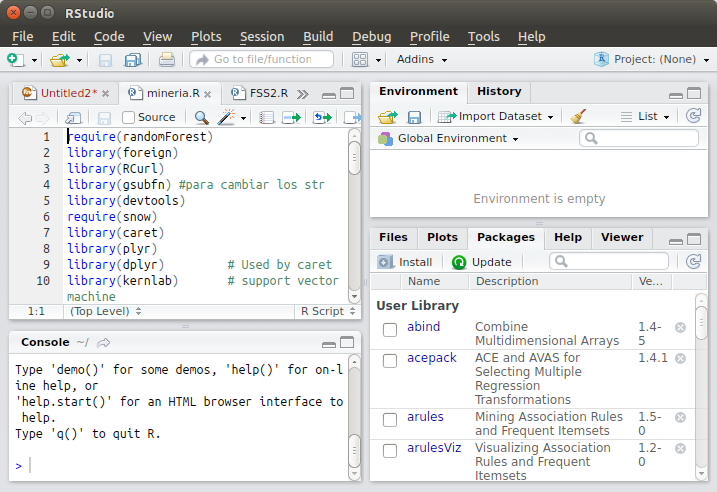
\includegraphics[height=.50\textwidth]{figs/RStudio.png}

\texttt{https://www.rstudio.com/}

\end{frame}

%%%%%%%%%%%%%%%%%%%%%%%%%%%%%%%%%%%%%%%%%%%%%%%%%%%%%%%%%%%%%%%%%%%%%%

\begin{frame}{RStudio?} %{What is the R language?}

Well known package authors work for RStudio.
%
\includegraphics{figs/RStudio-Logo-Blue-Gray-125.png}%[height=.15\textwidth]
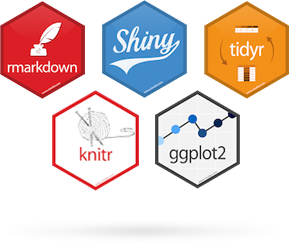
\includegraphics[height=.50\textwidth]{figs/r-packages.png}


\end{frame}


%%%%%%%%%%%%%%%%%%%%%%%%%%%%%%%%%%%%%%%%%%%%%%%%%%%%%%%%%%%%%%%%%%%%%%

\subsection[Packages]{Packages for Reproducible Research}

%%%%%%%%%%%%%%%%%%%%%%%%%%%%%%%%%%%%%%%%%%%%%%%%%%%%%%%%%%%%%%%%%%%%%%

\begin{frame}{Markdown} %{What is the R language?}

Markdown is a simple formatting syntax for authoring HTML, PDF, and MS Word documents. 

Extremely easy to learn and extensively used in RStudio.

\end{frame}

%%%%%%%%%%%%%%%%%%%%%%%%%%%%%%%%%%%%%%%%%%%%%%%%%%%%%%%%%%%%%%%%%%%%%%

\begin{frame}{knitr} %{What is the R language?}

knitr is an engine for dynamic report generation with R. It is a package in the statistical programming language R that enables integration of R code into LaTeX, LyX, HTML, Markdown, AsciiDoc, and reStructuredText documents.
\texttt{https://en.wikipedia.org/wiki/Knitr}

knitr extracts R code in the input document, evaluates it and writes the results to the output document

Rnw, Markdown, HTML and LaTeX

\texttt{http://yihui.name/knitr/}

\texttt{http://yihui.name/knitr/demo/minimal/}


\end{frame}


%%%%%%%%%%%%%%%%%%%%%%%%%%%%%%%%%%%%%%%%%%%%%%%%%%%%%%%%%%%%%%%%%%%%%%


\begin{frame}{Bookdown} %{What is the R language?}

It is way of authoring books with RMarkdown generating PDF, handouts and slides automatically.

\texttt{https://www.rstudio.com/resources/webinars/introducing-bookdown/}

\end{frame}


%%%%%%%%%%%%%%%%%%%%%%%%%%%%%%%%%%%%%%%%%%%%%%%%%%%%%%%%%%%%%%%%%%%%%%

\begin{frame}{Rnw} %{What is the R language?}

Inserts R into Latex documents.

\end{frame}

%%%%%%%%%%%%%%%%%%%%%%%%%%%%%%%%%%%%%%%%%%%%%%%%%%%%%%%%%%%%%%%%%%%%%%

\section[Collaborating and sharing]{Collaborating and sharing your research}

%%%%%%%%%%%%%%%%%%%%%%%%%%%%%%%%%%%%%%%%%%%%%%%%%%%%%%%%%%%%%%%%%%%%%%

\subsection{Git}{Git and GitHub}

%%%%%%%%%%%%%%%%%%%%%%%%%%%%%%%%%%%%%%%%%%%%%%%%%%%%%%%%%%%%%%%%%%%%%%

\begin{frame}{Git} %{What is the R language?}

Git 

\texttt{https://en.wikipedia.org/wiki/R\_(programming\_language)}
\end{frame}

%%%%%%%%%%%%%%%%%%%%%%%%%%%%%%%%%%%%%%%%%%%%%%%%%%%%%%%%%%%%%%%%%%%%%%

\begin{frame}{GitHub} %{What is the R language?}

GitHub 

\texttt{www.github.com}

Publish Websites, etc.

\end{frame}


%%%%%%%%%%%%%%%%%%%%%%%%%%%%%%%%%%%%%%%%%%%%%%%%%%%%%%%%%%%%%%%%%%%%%%
%%%%%%%%%%%%%%%%%%%%%%%%%%%%%%%%%%%%%%%%%%%%%%%%%%%%%% Conclusions %%%
%%%%%%%%%%%%%%%%%%%%%%%%%%%%%%%%%%%%%%%%%%%%%%%%%%%%%%%%%%%%%%%%%%%%%%


\section{Conclusions}
%%%%%%%%%%%%%%%%%%%%%%%%%%%%%%%%%%%%%%%%%%%%%%%%%%%%%%%%%%%%%%%%%%%%%%

\begin{frame}{Conclusions} %{What is the R language?}

\begin{itemize}
  \item Learn Bash and other tools for it: awk, make, sort, 
  \item Learn  Git, R or Python.
  \item If you use R/Python for your research automate as much as possible. It is much easier to modify.
  \item Try to stick to Open/libre software GNU/Linux, R, Python, etc.
\end{itemize}

\end{frame}


\end{document}
